\chapter{Einleitung}
Die digitale Technik und ein hoher Grad an Individualität nehmen einen immer höheren Stellenwert in der Lehre ein. 
Eine flexible Verteilung der Lernzeiten können das Lernen auch ohne Präsenzelemente stattfinden lassen, dies kann z.B. durch Videoaufzeichnungen der Lehrveranstaltung  erreicht werden.
Durch asynchronische und synchronische Lernphasen können einzelne Lernschritte zeitgleich, beispielsweise durch Ideenfindungen in Chats oder zeitverschoben durch individuelle Reflexionen ablaufen.
Ein ortsunabhängiges gemeinsames Bearbeiten von Aufgabenstellungen erfolgt durch eine virtuelle Vernetzung. Es können Programmieraufgaben zusammen per Livesharing bearbeitet und gelöst werden. Mithilfe von Virtual Reality Anwendungen können schwer zugängliche reale Objekte lösbar gemacht werden. Objekte in der Medizin können für Lernende durch virtuelles Mikroskopieren anschaulicher und zugänglicher dargestellt werden.
Diese Aspekte stellen bildungstechnologische Optionen dar, welche die Gestaltung des eigenen Lerntempos und 
der individuellen Art und Weise des Lernens
begünstigen. \parencite[170]{Lehner.2018} 
Um digitale und auf den Lernenden zugeschnittene Lernformate zu fördern, können Conversational Agents (CA) eingesetzt werden. 
Conversational Agents sind Systeme, die es Benutzern ermöglichen, mit ihnen unter der Verwendung natürlicher Sprache zu interagieren. \parencite[2 ff.]{Gnewuch.2017}
Beispielsweise können sie als virtueller Lehrassistent dienen, die durch die Beantwortung der Fragen der Schüler und die Bereitstellung 
von personalisiertem Feedback das Lerntempo an die Anforderungen jedes Lernenden anpassen.
Darüber hinaus sollen CAs nicht nur in der Tutorrolle fungieren, sondern auch die Rolle als Begleiter oder Moderator einnehmen. \parencite[46 ff.]{strohmann.2021} \parencite[10 ff.]{Strohmann.2018} 
Die Technologien wie Spracherkennung, Sofortantwort, Automatisierung und Prognostizierung ermöglichen dem Lernenden den Zugang zu einer personalisierten und sich schnell entwickelnden Ausbildung.
Somit wird die Zukunft der dialogorientierten Künstlichen Intelligenz im Bildungssektor als dynamische und zuversichtliche Unterstützung vorausgesagt. \parencite[1]{kumar.2021} \parencite[1]{pinker.2019}  

\section{Problemstellung} \label{Problemstellung}
Ein häufig genanntes Problem des digitalen Lernformates ist, dass die soziale Einbindung fehlt.
Eine Studie der Universität Würzburg mit ca. 4000 Studierenden zur Umstellung auf digitale Lehre während der Corona Pandemie bestärkt diese Erkenntnis. 
\footnote{\url{https://www.uni-wuerzburg.de/aktuelles/pressemitteilungen/single/news/studieren-in-coronazeiten-1}, aufgerufen am 23.10.2021}
Die Studierenden kritisieren, dass ihr Studium zu unpersönlich geworden ist. Alles, was sich an Kommunikation und emotionalem Austausch in der Präsenzlehre ergibt, muss im digitalen Setting explizit geschaffen werden, sodass ein Gefühl der sozialen Einbindung 
im digitalen Lehrformat entsteht. \parencite[90]{Uemminghaus.2021} 
Für ein erfolgreiches E-Learning ist die Fähigkeit zur Selbststeuerung des Lernprozesses besonders wichtig, da eine mangelnde Selbststeuerung den Lernerfolg gefährden kann und somit zu 
Motivationsdefiziten führt. \parencite[13]{berlinger.2002} \parencite[1]{weck.2020} 
Allerdings fehlt es oft an der Fähigkeit, selbstreguliertes Lernen\footnote{ Selbstorganisiert, selbstbestimmt, selbstreguliert, autonom, autodidaktisch, selbst gestalten oder selbstlernen sind mit dem Begriff der Selbststeuerung gleichzusetzen. \parencite[14 f.]{Dietrich.2007}} richtig zu gestalten. \parencite[1]{weck.2020} 
Mehrere der folgenden Kompetenzen müssen für ein effektives selbstreguliertes Lernen vorhanden sein und zum Einsatz kommen:
\begin{itemize}
    \item die Ziele angemessen zu setzen (z.B. Qualität und Quantität der zu erwerbenden Inhalte, Lernzeiten für die Erarbeitung der Inhalte, Tiefenverarbeitung bei der Wissensaneignung)
    \item die Einschätzung und Bewertung des Ist-Zustands und der Ist-Soll-Differenzen während des Versuchs das Ziel zu erreichen (z.B. realistische Einschätzung des eigenen Wissensstandes, bereits gemachter Lernfortschritte und des Abstandes zum Lernziel)
    \item das Wissen und die Fertigkeiten zur Reduzierung der Ist-Soll-Differenz (z.B. Planung von Lerneinheiten, ein Repertoire an Lernstrategie sowie das Know-How diese effektiv einzusetzen)
    \item die Motivation den Lernprozess zu initiieren und aufrechtzuerhalten durch die positive und affektive Einstellung zu Lerninhalten und des gesetzten Ziels
\end{itemize}
Zum Beispiel nützt die Kompetenz,
spezifische Ziele zu setzen sehr wenig, wenn nicht die Motivation und die konkreten Handlungen zur Erreichung der gesetzten Ziele vorhanden sind. \parencite[146 f.]{Nett.2019} 
Es wird somit mehr von den Lernenden gefordert als im herkömmlichen Setting, da die Lernenden bei der Nutzung von E-Learning Aktivitäten mehr 
Eigeninitiative und Selbstmotivation entwickeln müssen. \parencite[34]{marx.2006}
Ferner fehlt es oft an einer individuellen Betreuung beim E-Learning, die in Klassen mit vielen Schülern oder in Vorlesungen in der Universität nicht 
angeboten werden kann. 
Dadurch kann das Tempo und die Art und Weise in der Präsentation der Lerneinheit nicht auf jeden individuellen Lernenden abgestimmt werden,
wodurch die Aufmerksamkeit einzelner schwindet.
Also resultieren die Lerneinheiten oft im Frontalunterricht, da eine individuelle Lernbetreuung nicht skalierbar ist.
\parencite[1]{Oscar} \parencite[1]{Adel.2016}

Um den Motivationsproblemen der Lernenden entgegenzuwirken, können sich CAs auf eine natürliche Interaktion einlassen und das
Verständnis der Lernenden ähnlich wie Pädagogen aufbauen.\parencite[1]{winkler_hobert_salovaara_söllner_leimeister_2020}
Sofern jedem Lernenden ein eigener individueller CA zur Verfügung gestellt 
wird, spiegeln sich die pädagogischen Ansätze darin wider, dass der Lernende
mit einem CA als simulierter Peer eine soziale Interaktion durchlebt.
Durch die Interaktion mit einem menschenähnlichen Wesen ist der Lernende eine Vielzahl von
emotionalen Zuständen ausgesetzt. Der CA kann sich an den emotionalen Zustand, von dem sich der 
Lernende angesprochen fühlt, anpassen und so eine empathische Beziehung zum Lernenden aufbauen.\parencite[576 f.]{Kim.2006} 

Des Weiteren kann der CA als Ansprechpartner für die Gestaltung des Lernprozesses dienen.
Sofern Lernende mangelnde Selbstlernkompetenzen aufweisen, können die CAs den Aufbau eines Lernprozesses
begleiten und unterstützen, wobei hierbei die Charakterzüge des Lernenden eine große Bedeutung haben.
Daher sollte ein CA die Personenmerkmale wie sein persönliche Art und Weise des Lernens in die Gestaltung miteinbeziehen. \parencite[579]{Kim.2006} 
Folgend steht das Wissen über die Art und Weise, wie jeder Lernende beginnt, neue und komplexe Informationen aufzunehmen und zu verarbeiten 
in einer engen Beziehung zu den Motivationen und Einstellungen der Lernenden, wodurch die Stärke der 
Lernmotivation beeinflusst werden kann und bei einer Erhöhung sich positiv auf den Lernerfolg auswirkt.\parencite[30]{Schrader.2008} 

\section{Motivation und Zielsetzung} \label{Forschungsmotivation}

Neue Fortschritte intelligenter Technologien sind die Treiber der technischen Entwicklung von Chatbots und Conversational Agents.
Die Interaktion mit einem Lernsystem durch natürliche Sprache erhöht die 
Benutzerfreundlichkeit, da das Gefühl einer menschenähnlichen Interaktion 
erzeugt wird. \parencite[38-42]{Folstad_Brandtzaeg.2017} 
Einen Prototypen für ein solches Lernsystem stellen
Latham u.a (2010) vor. Oscar ist ein Conversational Intelligent Tutoring System (CITS).
Ein intelligentes Tutoringsystem sind Computerlernsysteme, die ihre Lerninhalte für eine Person personalisieren.
Ein CITS nutzt einen CA, um als Tutor aufzutreten. Oscar zielt darauf ab, einen menschenähnlichen
Tutor nachzuahmen, indem er den Lernstil des Studierenden während eines Nachhilfegesprächs im Bereich der
Structured Query Language (SQL) dynamisch einschätzt und sich an ihn anpasst.
Oscar nutzt Diagramme, Bilder und interaktive Lernvideos als Unterstützung zum Nachhilfegespräch.
Zur dynamischen Einschätzung des Lernstils nutzt Oscar Aspekte des Verhaltens und Verständnisses des Lernenden.
Zur anschließenden Klassifizierung des Lernstils verwendet Oscar das Lernstilinstrument Index of Learning Styles (ILS). \parencite[1 f.]{Oscar}
Der ILS-Fragebogen von Felder und Soloman (1991) ist ein Instrument zur Bewertung der Lernstiltypologie nach Felder und Silverman (1988). \parencite[2]{Felder.2002}

Durch die Bestimmung des Lernstils des Lernenden kann Oscar seine Nachhilfe für jeden einzelnen personalisieren, um die Effektivität der Nachhilfe zu verbessern.
Eine erste Pilotstudie mit 10 Teilnehmern wurde im Bereich der Betreuung von  Studierenden der Naturwissenschaften 
und der Ingenieurwissenschaften
durchgeführt. 
Die Ergebnisse der ersten Pilotstudie sind vielversprechend, da in drei Fällen die Genauigkeit der Schätzung des Lernstils bei 70 \% lag und im schlechtesten Fall bei 50 \%. \parencite[6 f.]{Oscar}
In einer weiteren Studie mit 65 Probanden hat Oscar den Lernstil aller Teilnehmer mit einer Genauigkeit zwischen 61 und 100 \% 
erzielt. \parencite[108]{Latham.2012} Dies zeigt, dass die Verwendung der Lernstiltypologie nach Felder und Silverman (1988)  eine Möglichkeit zur 
Identifikation des Lernstils bietet und für die vorliegende Arbeit von Relevanz ist.

Allerdings zielt die Lernstilermittlung von Oscar nur auf Studierende der Naturwissenschaften 
und der Ingenieurwissenschaften ab. Des Weiteren begrenzt sich die Identifikation des Lernstils auf ein Nachhilfegespräch
im Bereich der Datenbanksprache SQL. 
Genau hier ergibt sich eine Forschungslücke,
nämlich die Klassifikation des persönlichen Lernstils mithilfe eines CAs nicht nur auf eine Studienrichtung zu begrenzen,
sondern alle Lernende als Zielgruppe zu betrachten, ob in einer beruflichen Weiterentwicklung, 
als Schüler oder Studierender. Dazu ist es wichtig ein Setting zu erstellen,
welches nicht auf ein Dialog bezüglich eines bestimmten Studienfachs abzielt,
sondern eines allgemeinen und natürlichen Dialogs zwischen CA und Lernendem.
Zur Entwicklung des CAs wird das Open-Source Framework Rasa verwendet. Rasa nutzt 
Maschinelles Lernen für das Bauen von Chatbots. \parencite[25]{Kong.2021} 
Mithilfe von Maschinellem Lernen sollen IT-Systeme automatisch Muster und 
Zusammenhänge aus Daten lernen. \parencite[35]{deru.2020} 
Dies dient dazu, dass die Eingaben des Dialogs nicht exakt den, in dem Bot hinterlegten Ausdrücken, 
entsprechen müssen, sodass der Bot flexibler auf die Eingaben reagieren und antworten kann. \parencite[142]{Sieber.2019}

In dieser Bachelorarbeit wird ein Prototyp zur Bestimmung des individuellen Lernstils des Lernenden 
entwickelt, um die aufgeführte Forschungslücke zu reduzieren.
Der CA soll den persönlichen Lernstil des Lernenden anhand von identifizierten Merkmalen bezüglich seiner Lerneinstellung 
in einem Dialog automatisch klassifizieren können. Es wird die Taxonomie des Lernstils verwendet, da 
der Dialog auf den Fragen des ILS-Fragebogens basiert.
Die Items des Fragebogens stellen die zu identifizierenden Merkmale der Lerneinstellung des Lernenden dar.
Um den Motivationsproblemen der Lernenden entgegenzuwirken,
soll der Lernende durch die Kommunikation mit dem CA eine soziale Bindung aufbauen 
und eine Unterstützung im selbstregulierten Lernen in der Online Lehre erfahren.
Dazu soll geprüft werden, inwieweit der CA den Lernenden motiviert. 
Die Forschungsfragen der vorliegenden Arbeit sind folgende:

\begin{itemize}                 
    \item \textbf{RQ1:} \textit{\glqq Inwiefern ist es möglich, durch eine dialogbasierte Interaktion eines Lernenden in natürlicher Sprache mit einem persönlichen CA den individuellen Lernstil für den Lernenden zu bestimmen?\grqq{} }
    \item \textbf{RQ2:} \textit{\glqq Inwiefern kann das Motivationsverhalten des Lernenden durch die Interaktion mit einem CA beeinflusst werden?\grqq{} }
\end{itemize}

Ein weiterer Aspekt dieser Arbeit ist es zu untersuchen, inwiefern es möglich ist, Gamification und CAs miteinander zu verbinden.
Gamification ist definiert als eine Technik,
in der Spielelemente in nicht spielerische Kontexte eingebunden werden
und dadurch die Motivation von Lernenden erhöht. \parencite[4]{Arai.2014} \parencite[1]{Sailer.2013}
Krause u.a. (2015) haben die Auswirkung von Gamification auf den Lernerfolg 
von Studierenden untersucht. Die Studienteilnehmer wurden in spiellose und in
spielgebundene Gruppen eingeteilt. Die Gruppen wurden bezüglich
des Kriteriums der Quiz-Richtigkeit analysiert. Eine ihrer Forschungsfragen war, 
ob Gamification den Lernerfolg von Studierenden während eines Online-Kurses 
unterstützt. Das Ergebnis der Studie ergab einen signifikanten Unterschied zwischen
beiden Gruppen. Die Gruppe mit der Einbindung von Spielelementen hat ein 12,5 \%iges 
besseres Ergebnis bei der Quiz-Auswertung erreicht. \parencite[3 ff.]{Krause.2015}\\
Die Möglichkeit einer Verbindung zwischen Gamification und CAs herzustellen, zeigen Johnson u.a. (2022)
mit der Erstellung des Telegrammbots \glqq Escapeling\grqq{}.
Escapeling zielt darauf ab,
die Englischkenntnisse außerhalb des Klassenzimmers zu verbessern.
Lernende der Mittelstufe können gemeinsam in einem spielerischen
Escape-Room-Szenario üben, in dem sie verschiedene Aufgaben lösen müssen.
Durch spielintere Erfolgs- und Erzählgeschichten wird der Spieler dazu angeregt,
das langfristige Ziel, die Flucht aus dem Schiff, zu verfolgen. \parencite[1]{Johnson.2022}

Quiz-Apps werden of zu Unterhaltungszwecken eingesetzt und sind aufgrund des hohen 
Spielspaßes sehr beliebt. \parencite[487]{Söbke.2015}
Verschiedene Quiz-Apps sind für Lernzwecke entwickelt worden und werden kommerziell angeboten. \footnote{Socrative: \url{https://www.socrative.com/}, aufgerufen am 06.01.2022} \footnote{Quizlet: \url{https://quizlet.com/de}, aufgerufen am 06.01.2022}
Darüber hinaus sind Quiz-Apps aus wissenschaftlichen Projekten Gegenstand der Forschung. Diese
weisen motivationssteigernde und lernfördernde Effekte auf Studierende nach. \parencite[1]{Pechenkina.2017} \parencite[2]{Roediger.2011} \\
Um den Unterhaltungs- und Spieltrieb des Lernenden zu nutzen, soll der Prototyp dieser Arbeit mithilfe eine Quizes
in einer zweiten Interaktion zwischen Prototyp und Lernendem den persönlichen Lernstil ein weiteres Mal
bestimmen. Zusätzlich zu den zwei wesentlichen Forschungsfragen soll die
Möglichkeit zur Bestimmung des persönlichen Lernstils mithilfe eines Quizes sowie die Auswirkung 
dieser Interaktion auf die Lernmotivation untersucht werden. 

Diese Arbeit wird parallel zu dem dreijährigen Projekt StudyBuddy erstellt. Das Projekt StudyBuddy hat das Ziel, einen virtuellen Lernbegleiter für den Lernenden zu gestalten.
Dieser Lerncompanion soll den Lernenden während seines Lernprozesses begleiten und unterstützen, sodass frühzeitig Wissens- und Verständnislücken identifiziert und behoben werden
sowie Empfehlungen, die individuell auf den Lernenden zugeschnitten sind, gegeben werden. Dadurch soll langfristig der Lernerfolg erhöht und die Abbruchquote in Weiterbildungsmaßnahmen gesenkt werden. \footnote{\url{https://study-buddy-research.de/}, aufgerufen am 23.10.2021}

\section{Wissenschaftliche Vorgehensweise} \label{Vorgehensweise}
Um das Forschungsziel zu erreichen, wird ein Design Science Research (DSR) Ansatz 
nach Hevner (2007) angewendet. Dieser Ansatz eignet sich, um mit 
einer wissenschaftlichen Methode ein praktisches Problem zu lösen. \parencite[91]{Hevner.2007}
Gregor und Hevner (2013) bezeichnen die DSR-Methode als ein Paradigma der Informationssysteme (IS),
welcher damit einen geeigneten Ansatz für die Beantwortung der Forschungsfragen aufweist. \parencite[337]{Gregor.2013}
Außerdem 
soll durch die Gestaltung und Bewertung des neuen Forschungsartefakts 
ein Beitrag zum Forschungsbestand geleistet werden.
Im DSR gibt es drei verschiedene Arten von Forschungsartefakten.
Level-1-Artefakte beziehen sich auf einen bestimmten Anwendungskontext, wie 
z.B. ein Softwareprodukt, ein Prototyp oder ein eingeführter Prozess. 
Level-2-Artefakte beziehen sich auf Konstrukte, Methoden, Modelle, Gestaltungsrichtlinien
und technologische Regeln.
Level-3-Artefakte sind vollständige entwickelte Designtheorien, welche weitreichendes und 
ausgereiftes Wissen darstellen.  \parencite[342]{Gregor.2013}
Der in dieser Arbeit zu entwickelnde Prototyp zur Bestimmung des persönlichen Lernstils lässt sich als Level-1-Artefakt kategorisieren.
Die DSR Methode besteht aus einem Prozess aus drei iterativen Zyklen, welche sich 
in Relevance Zyklus, Design Zyklus und Rigor Zyklus unterteilen (vgl. Abbildung \ref{fig:DSR}). \parencite[88]{Hevner.2007}
\begin{figure}[H]
    \centering
    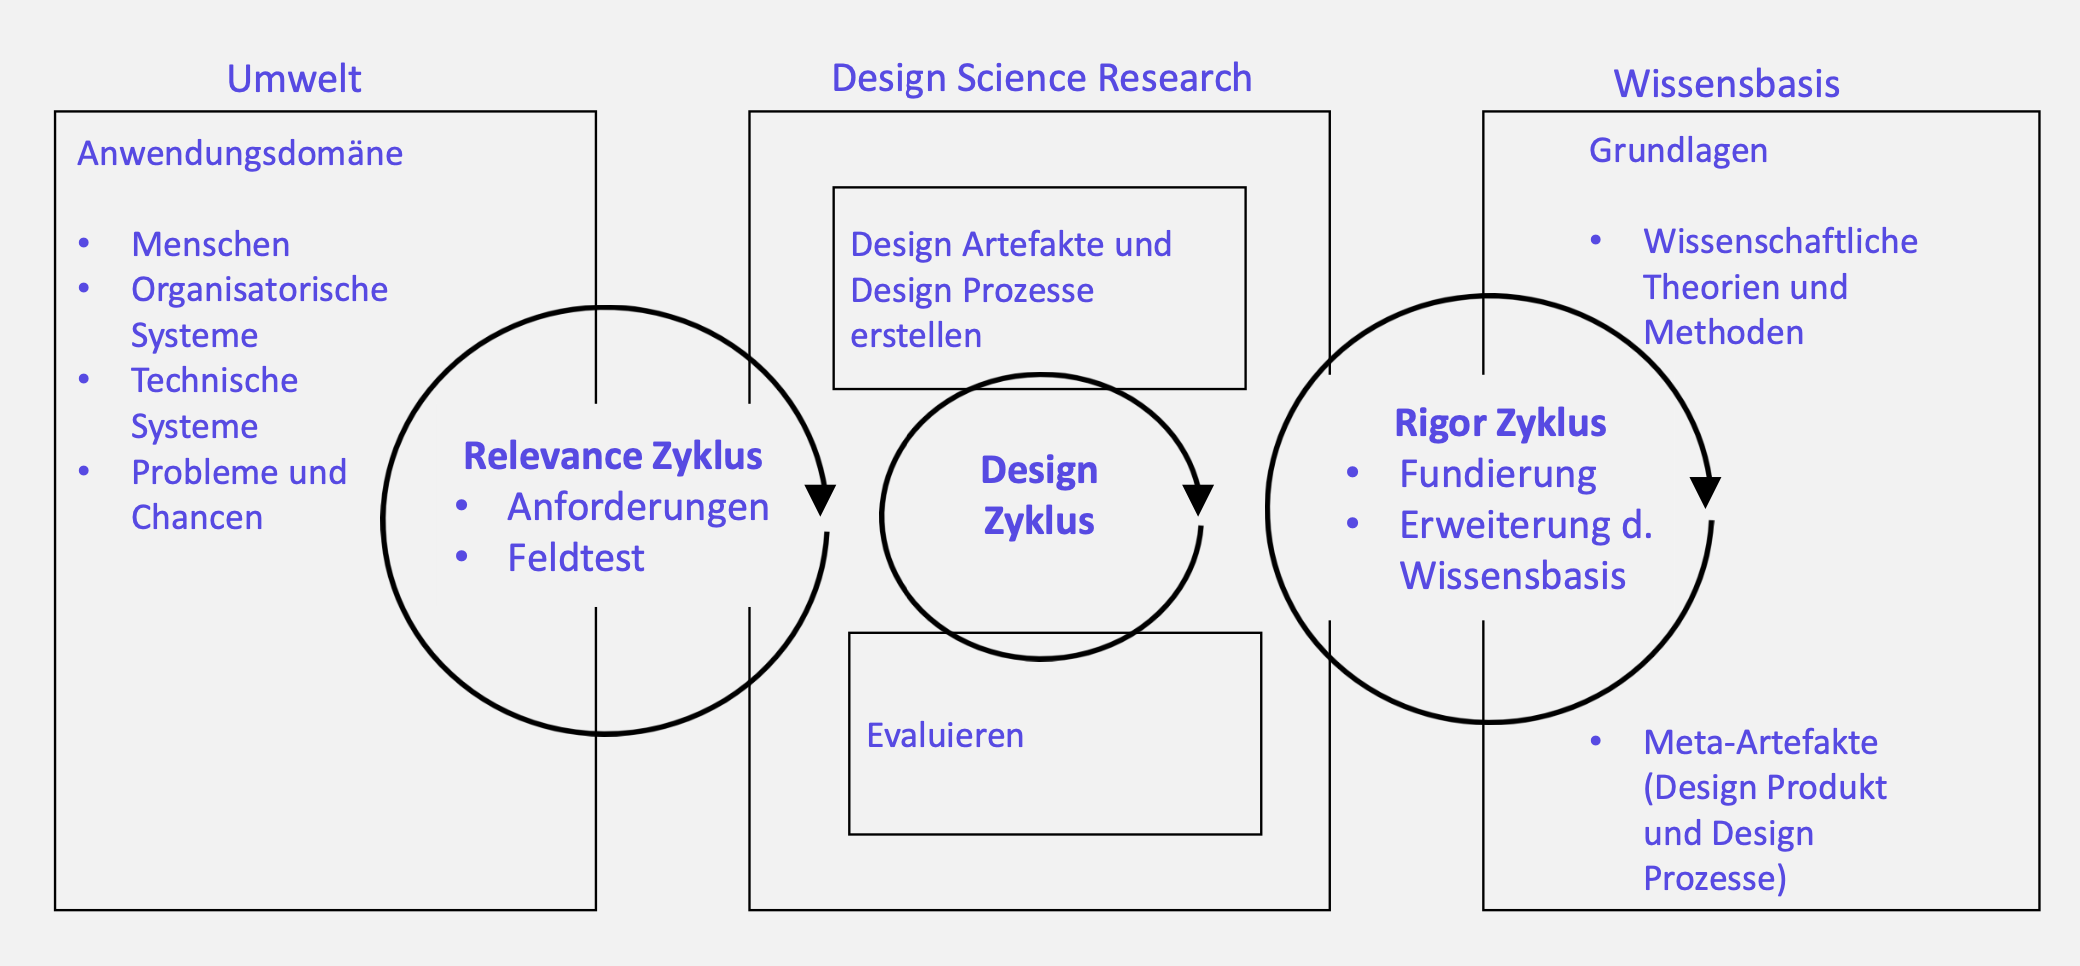
\includegraphics[width=1\linewidth]{images/Hevner.png}
    \caption[Design Science Research]{Design Science Research (eigene Darstellung, in Anlehnung an \parencite[88]{Hevner.2007})}
    \label{fig:DSR}
\end{figure}
Das Vorgehen der vorliegenden Arbeit basiert auf den eben genannten Zyklen.
\begin{itemize}
    \item \textbf{Relevance Zyklus:} \\
Hevner (2007) ist der Meinung, dass gute DSR Forschung mit der Identifizierung 
und Darstellung von Problemen in einem tatsächlichen Anwendungskontext beginnt.
Des Weiteren werden Akzeptanzkriterien für die Bewertung des Forschungsergebnisses definiert.
Abschließend werden in einem Feldtest die Ergebnisse evaluiert und bestimmt, ob 
eine weitere Iteration für die Anpassung der zuvor aufgestellten Anforderungen nötig ist. \parencite[89]{Hevner.2007}
Die vorliegende Arbeit stellt einen Ansatz für eine Identifikation des persönlichen Lernstils
eines Lernenden durch einen CA dar. Dazu wird ein Prototyp konstruiert.
Des Weiteren werden Bewertungskriterien aufgestellt, die prüfen, inwiefern die 
Interaktion mit dem Prototypen die Lernmotivation des Lernenden beeinflussen kann.
\item \textbf{Rigor-Zyklus:}\\
Eine umfangreiche Wissensbasis wissenschaftlicher Theorien und technischer Modelle stellen eine
Grundlage für Projekte der DSR Forschung. 
Der Rigor-Zyklus kann  
auf Wissen aus der Vergangenheit während des Forschungsprozesses 
zurückgreifen. Die Rigorosität der Forschung 
im DSR beruht auf der geschickten Auswahl und Anwendung geeigneter Theorien und Methoden. \parencite[90]{Hevner.2007}
Deshalb werden in der vorliegenden Arbeit relevante historische 
Theorien zur Lerntypologie vorgestellt,
um die ausgewählte Lerntypologie des Lernstils sowie das ausgewählte
ILS-Instrument von Felder und Soloman (1991), welches auf dem Lernstilmodell
 von Felder und Silverman (1988) basiert, zu begründen.
Für die Konzeption des Prototyps wird der aktuelle Stand der Forschung bezüglich der 
Themenkombination \glqq CA im Lehrformat\grqq{} sowie \glqq CA zur Identifikation des Lernstils\grqq{} untersucht.
Ferner werden für die Gestaltung des CAs Guidelines aufgestellt, welche sich 
auf identifizierte Aspekte der Wissensbasis zurückführen lassen.
Zur Ansammlung der benötigten Informationen wurde  
eine unsystematische Literaturanalyse genutzt.

\item \textbf{Design-Zyklus:}\\
Der Design Zyklus ist der Kernprozess eines DSR Forschungsprojekts. Dieser Zyklus stellt einen Ablauf 
von Forschungsaktivitäten dar, um Artefakte zu konstruieren und anschließend zu bewerten. \parencite[90 f.]{Hevner.2007}
Der Prototyp zur Identifikation des persönlichen Lernstils wird mithilfe einer Online-Umfrage evaluiert und weiterentwickelt.
\end{itemize}

\section{Aufbau der Arbeit}

Um den dargestellten Forschungsfragen nachzugehen, folgt die vorliegende Arbeit folgender Struktur:\\
Nach dieser Einleitung folgen \textbf{im 
zweiten Kapitel} die theoretischen Grundlagen des Lernens.
Es wird auf die Definitionen des Lernens, des digitalen Lernens und des selbstregulierten Lernens
eingegangen. Zur Beantwortung von RQ2 wird die Entstehung der Lernmotivation erläutert
sowie das ARCS-Modell zur Messung der Lernmotivation vorgestellt.
Für die Begründung der Wahl der Lerntypologie des Lernstils und des Modells von Felder und Silverman (1988), 
bedarf es vorerst einer Begriffsabgrenzung von Lerntypologien und eines Überblicks bekannter Modelle der Lerntypologien.
\textbf{Das dritte Kapitel} gibt eine Einführung in den Themenbereich der Chatbots.
Um die Chatbot-Begriffe abzugrenzen, folgen Definitionen  zum Chatbot,
zum Conversational Agenten
 und zum Virtual Companion.
Anschließend werden Informationen zum 
Natural Language Processing und zum Maschinellem Lernen aufgeführt, um 
zu klären inwiefern das Maschinelle Lernen Conversational Agents unterstützen. 
Zum Schluss des dritten Kapitels wird der aktuelle Stand der Forschung zu CAs dargestellt,
die eine mögliche Einschätzung vom Lernstil bei Lernenden untersucht haben oder in Lehrformaten
eingesetzt wurden. Dies dient der Erfassung der bestehenden Wissensbasis.
Das Kapitel zwei und drei stellen den theoretischen Teil der Arbeit dar. Die folgenden Kapitel
beziehen sich auf den Praxisteil der vorliegenden Arbeit.
\textbf{In dem vierten Kapitel} wird der Prototyp zur Identifikation des persönlichen Lernstils vorgestellt. 
Dabei wird zuerst auf das verwendete Framework Rasa eingegangen. Danach folgt die
Vorstellung des Prototyps, wobei vertieft auf 
die Dialog- und die Quiz-Spielgestaltung zwischen Lernendem und CA eingegangen wird.
\textbf{Das fünfte Kapitel} stellt die Evaluierung des Prototyps dar. 
Zuerst wird der Aufbau des Fragebogens erläutert. Anschließend folgt die Auswertung, welche nötig ist, um
RQ1 und RQ2 zu beantworten.
Abschließend folgt \textbf{im sechsten Kapitel} eine Zusammenfassung sowie 
eine kritische Würdigung des neu gewonnenen Wissens und
es wird ein Ausblick für weitere Forschungen aufgezeigt.

Bezogen auf die in Kapitel \ref{Vorgehensweise} beschriebene Vorgehensweise der Arbeit nach Hevner (2007),
spiegelt sich der Relevance Zyklus in der aufgeführten Problemstellung (vgl. Kapitel \ref{Problemstellung})
und in der Forschungsmotivation (vgl. Kapitel \ref{Forschungsmotivation}) wider.
Die unsystematische Literaturanalyse, 
welche erstens zur Analyse der Modelle der Lerntypologien, zweitens zum Stand der Forschung bezüglich 
bestehender CAs zur Lernstilklassifikation und CAs im Lehrformat, drittens zur
Aufstellung von Gestaltungsrichtlinien 
für den Prototypen (vgl. Kapitel \ref{AnalyseLernstilmodelle}, \ref{StandderForschung} und \ref{Gestaltungsrichtlinien})
genutzt wurde, repräsentieren wie die Studie zum Prototypen (vgl. Kapitel \ref{Kapitel5}) den Rigor Zyklus zur Generierung von neuem Wissen und neuen Erfahrungen.
Der Design Zyklus wird durch die Vorstellung und Evaluierung des Prototyps dargestellt (vgl. Kapitel \ref{VorstellungPrototyp} \& \ref{Kapitel5.2}).
